\documentclass[a4paper]{article}
\usepackage{tikz}
\begin{document}
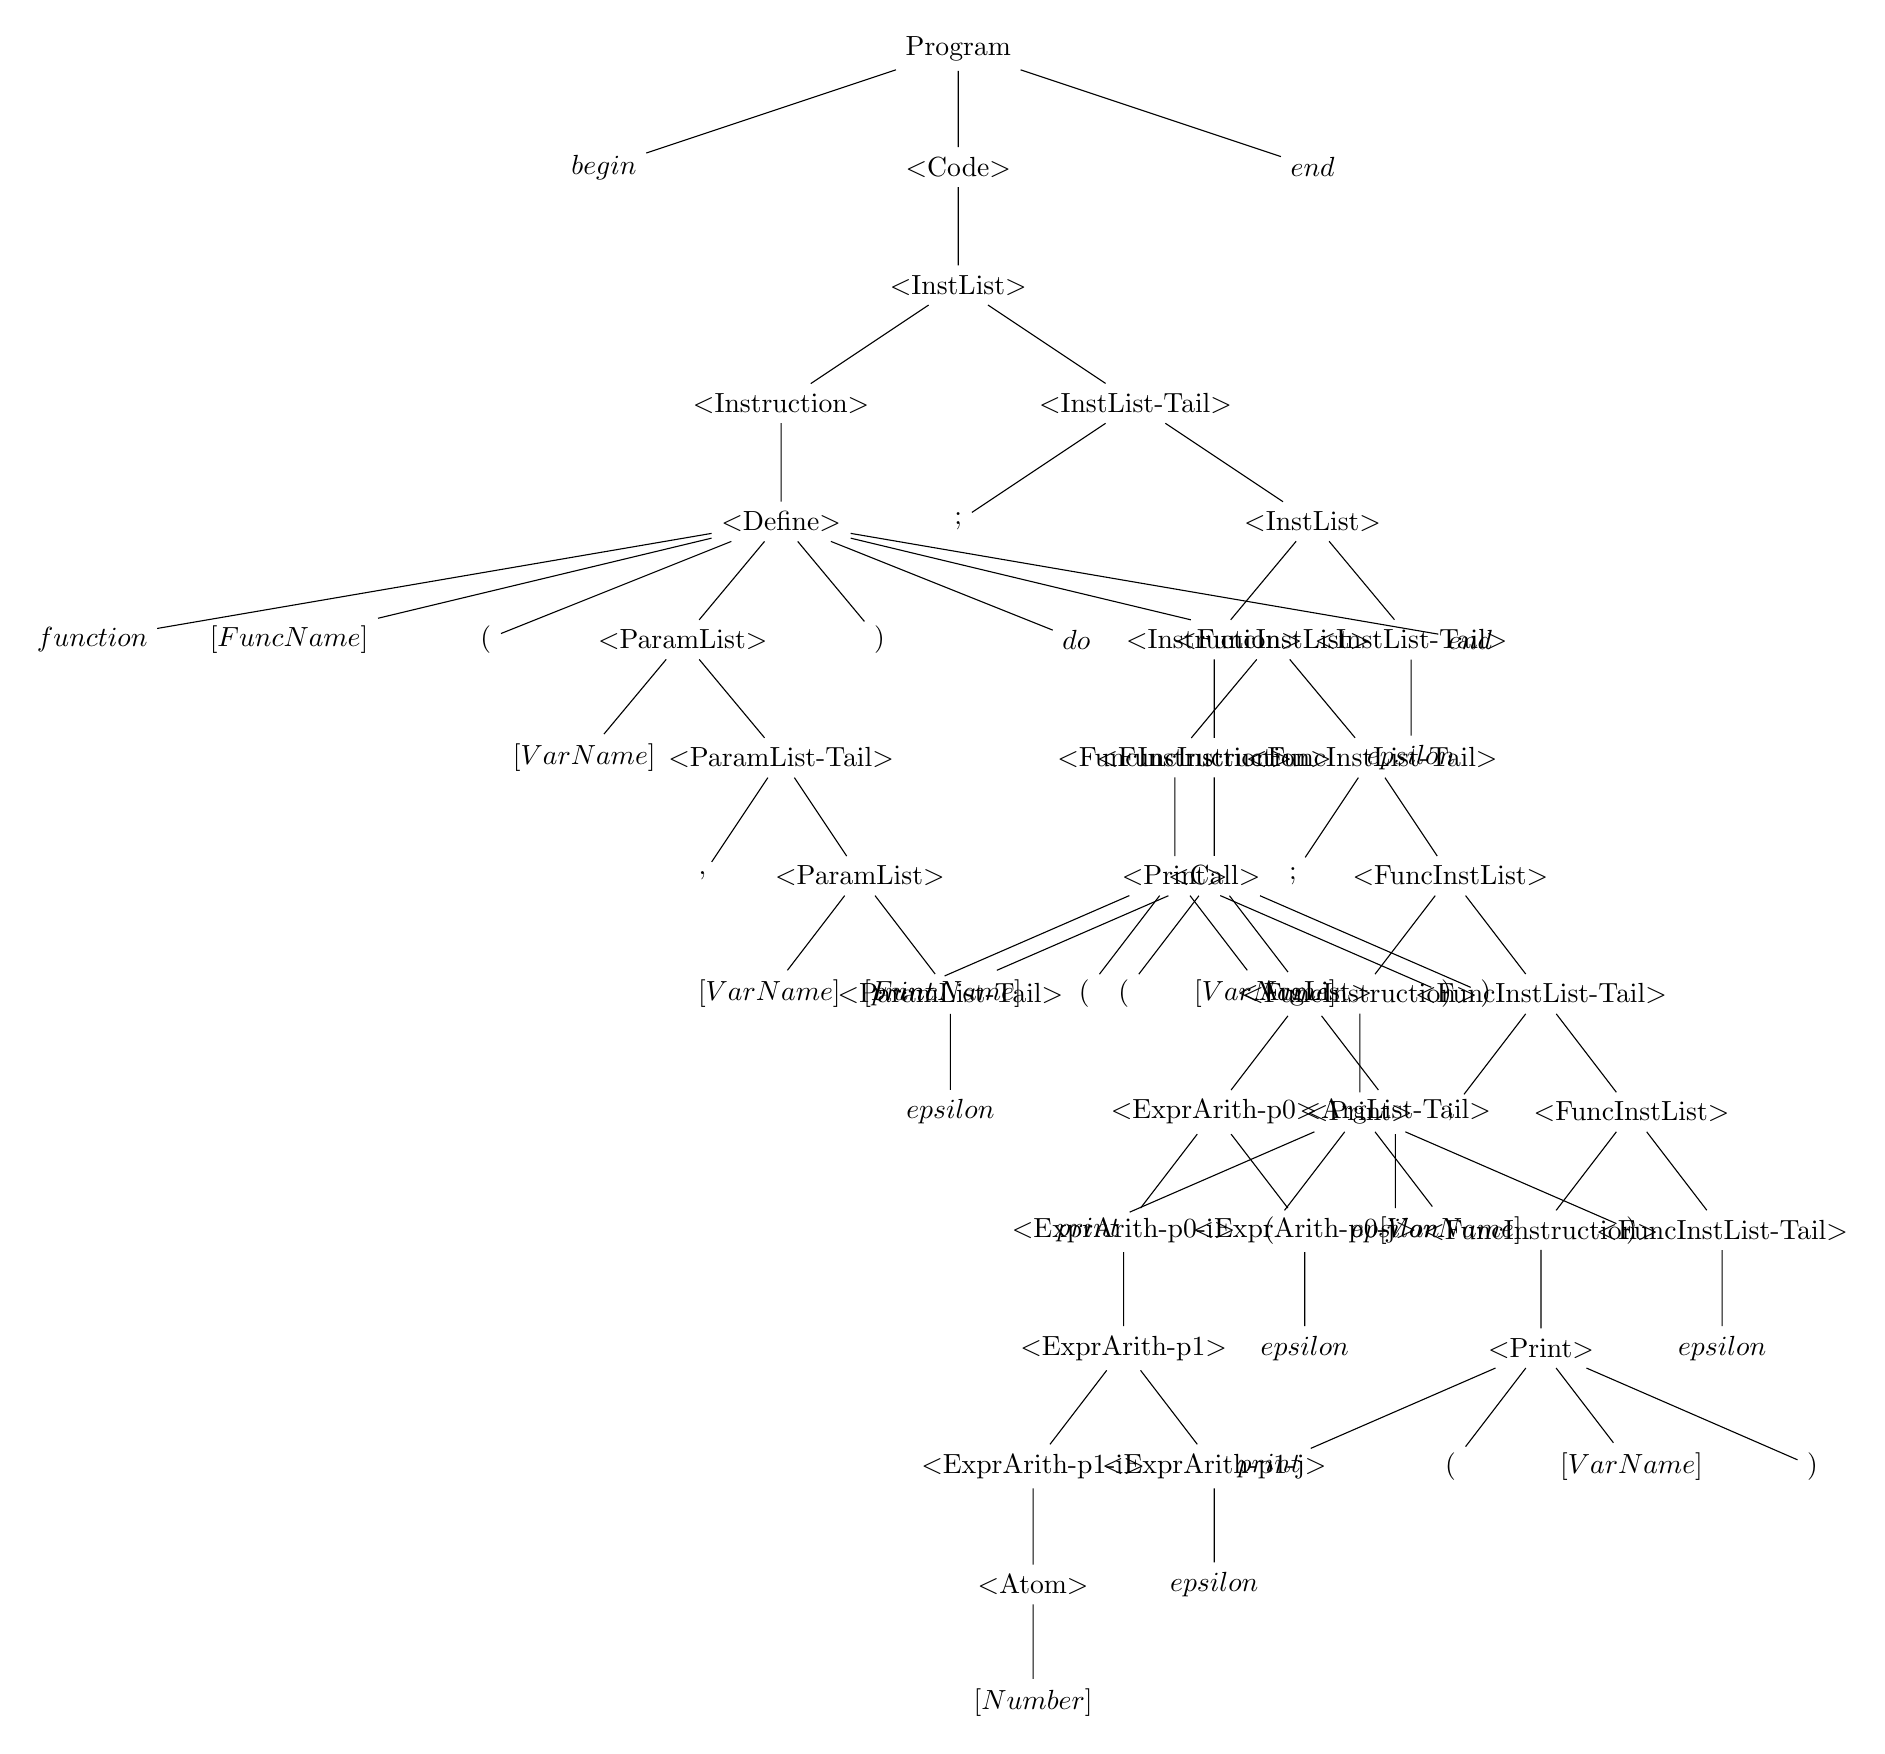
\begin{tikzpicture}[level 1/.style={sibling distance=45mm},level 2/.style={sibling distance=45mm},
 level 3/.style={sibling distance=45mm},level 4/.style={sibling distance=45mm},
 level 5/.style={sibling distance=25mm},level 6/.style={sibling distance=25mm},
 level 7/.style={sibling distance=20mm},level 8/.style={sibling distance=23mm}]
\node {Program}
child { node {$begin$}}
child { node {$<$Code$>$}
child { node {$<$InstList$>$}
child { node {$<$Instruction$>$}
child { node {$<$Define$>$}
child { node {$function$}}
child { node {$[FuncName]$}}
child { node {$($}}
child { node {$<$ParamList$>$}
child { node {$[VarName]$}}
child { node {$<$ParamList-Tail$>$}
child { node {$,$}}
child { node {$<$ParamList$>$}
child { node {$[VarName]$}}
child { node {$<$ParamList-Tail$>$}
child { node {$epsilon$}}
}
}
}
}
child { node {$)$}}
child { node {$do$}}
child { node {$<$FuncInstList$>$}
child { node {$<$FuncInstruction$>$}
child { node {$<$Print$>$}
child { node {$print$}}
child { node {$($}}
child { node {$[VarName]$}}
child { node {$)$}}
}
}
child { node {$<$FuncInstList-Tail$>$}
child { node {$;$}}
child { node {$<$FuncInstList$>$}
child { node {$<$FuncInstruction$>$}
child { node {$<$Print$>$}
child { node {$print$}}
child { node {$($}}
child { node {$[VarName]$}}
child { node {$)$}}
}
}
child { node {$<$FuncInstList-Tail$>$}
child { node {$;$}}
child { node {$<$FuncInstList$>$}
child { node {$<$FuncInstruction$>$}
child { node {$<$Print$>$}
child { node {$print$}}
child { node {$($}}
child { node {$[VarName]$}}
child { node {$)$}}
}
}
child { node {$<$FuncInstList-Tail$>$}
child { node {$epsilon$}}
}
}
}
}
}
}
child { node {$end$}}
}
}
child { node {$<$InstList-Tail$>$}
child { node {$;$}}
child { node {$<$InstList$>$}
child { node {$<$Instruction$>$}
child { node {$<$FuncInstruction$>$}
child { node {$<$Call$>$}
child { node {$[FuncName]$}}
child { node {$($}}
child { node {$<$ArgList$>$}
child { node {$<$ExprArith-p0$>$}
child { node {$<$ExprArith-p0-i$>$}
child { node {$<$ExprArith-p1$>$}
child { node {$<$ExprArith-p1-i$>$}
child { node {$<$Atom$>$}
child { node {$[Number]$}}
}
}
child { node {$<$ExprArith-p1-j$>$}
child { node {$epsilon$}}
}
}
}
child { node {$<$ExprArith-p0-j$>$}
child { node {$epsilon$}}
}
}
child { node {$<$ArgList-Tail$>$}
child { node {$epsilon$}}
}
}
child { node {$)$}}
}
}
}
child { node {$<$InstList-Tail$>$}
child { node {$epsilon$}}
}
}
}
}
}
child { node {$end$}}
;
\end{tikzpicture}
\end{document}
